\documentclass[12pt, titlepage]{article}

\usepackage{booktabs}
\usepackage{tabularx}
\usepackage{float}
\usepackage{hyperref}
\usepackage{graphicx}
\hypersetup{
    colorlinks,
    citecolor=black,
    filecolor=black,
    linkcolor=red,
    urlcolor=blue
}
\usepackage[round]{natbib}

\title{SE 3XA3: Test Report\\Namcap}

\author{Team 2, VPB Game Studio
		\\ Prajvin Jalan (jalanp)
		\\ Vatsal Shukla (shuklv2)
		\\ Baltej Toor (toorbs)
}

\date{\today}

%% Comments

\usepackage{color}

\newif\ifcomments\commentstrue

\ifcomments
\newcommand{\authornote}[3]{\textcolor{#1}{[#3 ---#2]}}
\newcommand{\todo}[1]{\textcolor{red}{[TODO: #1]}}
\else
\newcommand{\authornote}[3]{}
\newcommand{\todo}[1]{}
\fi

\newcommand{\wss}[1]{\authornote{blue}{SS}{#1}}
\newcommand{\ds}[1]{\authornote{red}{DS}{#1}}
\newcommand{\mj}[1]{\authornote{red}{MSN}{#1}}
\newcommand{\cm}[1]{\authornote{red}{CM}{#1}}
\newcommand{\mh}[1]{\authornote{red}{MH}{#1}}

% team members should be added for each team, like the following
% all comments left by the TAs or the instructor should be addressed
% by a corresponding comment from the Team

\newcommand{\tm}[1]{\authornote{magenta}{Team}{#1}}


\begin{document}

\maketitle

\pagenumbering{roman}
\tableofcontents
\listoftables
\listoffigures

\begin{table}[bp]
\caption{\bf Revision History}
\begin{tabularx}{\textwidth}{p{3cm}p{2cm}X}
\toprule {\bf Date} & {\bf Version} & {\bf Notes}\\
\midrule
2016-12-08 & 1.0 & Completion of Functional Requirements Evaluation\\
2016-12-08 & 1.1 & Completion of Unit Testing Section\\
\bottomrule
\end{tabularx}
\end{table}

\newpage

\pagenumbering{arabic}

This document ...

\section{Functional Requirements Evaluation}

\subsection{Game Functionality Testing}

\paragraph{}
A Robot (automated) unit testing class was implemented and used to test the mechanics of the game.

\begin{enumerate}

\item{GFT1\\}

Type: Functional, Dynamic, Automated
					
Initial State: Application is displaying the main menu page
					
Input: Cursor clicked on Start Game button
					
Expected Output: New game is started and window is changed to reflect a new game state

Output: New game was started and window was changed to reflect a new game state

Result: PASS


\item{GFT11\\}

Type: Functional, Dynamic, Automated
					
Initial State: Within game state
					
Input: Escape button pressed
					
Expected Output: Application must pause and ask user if they want to quit

Output: Game was paused and user was asked to quit or continue

Result: PASS

\end{enumerate}

\subparagraph{Player Movement/Collision Testing}

\begin{enumerate}

\item{GFT2\\}

Type: Functional, Dynamic, Automated
					
Initial State: Within the game state
					
Input: Arrow keys
					
Expected Output: Player moves in the respective direction (if path is clear)

Output: Player moved in the respective direction when path was clear
					
Result: PASS

\item{GFT3\\}

Type: Functional, Dynamic, Automated
					
Initial State: Player comes in contact with wall
					
Input: No input
					
Expected Output: Player stops moving when coming in contact with the wall

Output: Player's x and y coordinates were not changed when in contact with the wall

Result: PASS

\item{GFT4\\}

Type: Functional, Dynamic, Automated
					
Initial State: Player comes in contact with enemy
					
Input: No input
					
Expected Output: If player has more than 1 life, decrement lives. If player has one life, end game.

Output: Player's life was decremented by 1 when player had more than one life. The game was ended if player was on their last life.

Result: PASS

\item{GFT6\\}

Type: Functional, Dynamic, Automated
					
Initial State: Player comes in contact with dots
					
Input: Arrow keys
					
Expected Output: Dot disappears after collection

Output: Dot disappeared afer player colletcted it

Result: PASS

\item{GFT7\\}

Type: Functional, Dynamic, Automated
					
Initial State: Player collects the big dot
					
Input: Arrow keys
					
Expected Output: Big dot disappears after collection

Output: Big dot disappeared after player collected it

Result: PASS

\item{GFT8\\}

Type: Functional, Dynamic, Automated
					
Initial State: Player collects the big dot
					
Input: Arrow keys
					
Expected Output: Player is able to collide with enemies

Output: Player does not lose any lives when colliding with enemy

Result: PASS

\end{enumerate}

\subparagraph{Enemy Movement/Collision Testing}

\begin{enumerate}

\item{GFT5\\}

Type: Functional, Dynamic, Automated
					
Initial State: Within the game state
					
Input: No input
					
Expected Output: Enemies move on a valid path

Output: Enemy does not go through barriers

Result: PASS

\item{GFT9\\}

Type: Functional, Dynamic, Automated
					
Initial State: Player collects the big dot
					
Input: No input
					
Expected Output: Enemies change colour

Output: Enemies changed colours

Result: PASS

\item{GFT14\\}

Type: Functional, Dynamic, Automated
					
Initial State: Player collides with enemy after collection of big dot
					
Input: Arrow keys
					
Expected Output: Enemy is removed from game and respawned back to their original cell

Output: Enemy is respawned back to the center of the game

Result: PASS

\end{enumerate}

\subparagraph{Scoring Testing}

\begin{enumerate}

\item{GFT10\\}

Type: Functional, Dynamic, Automated
					
Initial State: Player collects all dots
					
Input: Arrow keys
					
Expected Output: Game over screen is activated

Output: Player's score is displayed along with the Game Over screen

Result: PASS

\item{GFT12\\}

Type: Functional, Dynamic, Automated
					
Initial State: Player collects dot
					
Input: Arrow keys
					
Expected Output: The points are increased

Output: Player's score is increased by 100

Result: PASS

\item{GFT13\\}

Type: Functional, Dynamic, Automated
					
Initial State: Player collects big dot
					
Input: Arrow keys
					
Expected Output: The points are increased at twice the rate

Output: Player's score is increased by 200

Result: PASS

\end{enumerate}

\section{Nonfunctional Requirements Evaluation}

\subsection{Usability}
		
\subsection{Performance}

\subsection{etc.}
	
\section{Comparison to Existing Implementation}	

This section will not be appropriate for every project.

\section{Unit Testing}

Unit Testing for Namcap was done using Java's JUnit testing suite, and results of all tests were written and summarized to a text file. If any tests failed, the exception would be included so the development team could analyze and repair any errors. Figure \ref{FigUTR} is an example of the text file.

\begin{figure}[H]
\centering
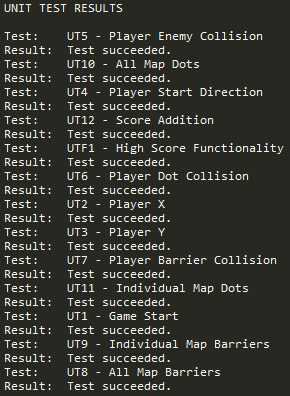
\includegraphics[width=0.5\textwidth]{UnitTestResults.png}
\caption{Unit Test Results}
\label{FigUTR}
\end{figure}

{\bf Test Cases}

\begin{enumerate}

\item{UT1\\}

Type: Unit, Static, Automated
					
Initial State: Application is displaying the main menu page
					
Input: Start Game button action is performed
					
Expected Output: New game is started and window is changed to reflect a new game state
					
Output: New window (game board) successfully opened

JUnit Test Result: PASS

\item{UT2\\}

Type: Unit, Static, Automated
					
Initial State: Player is in starting position at the start of the game
					
Input: Current X accessor method for the player
					
Expected Output: 200 (start X position)
					
Output: 200

JUnit Test Result: PASS

\item{UT3\\}

Type: Unit, Static, Automated
					
Initial State: Player is in starting position at the start of the game
					
Input: Current Y accessor method for the player
					
Expected Output: 300 (start Y position)
					
Output: 300

JUnit Test Result: PASS

\item{UT4\\}

Type: Unit, Static, Automated
					
Initial State: Player is in starting position at the start of the game
					
Input: Current direction of the player
					
Expected Output: 'R' (player starting direction)
					
Output: 'R'

JUnit Test Result: PASS

\item{UT5\\}

Type: Unit, Static, Automated
					
Initial State: Player is in starting position at the start of the game
					
Input: PlayerX, PlayerY, EnemyX, EnemyY (200,300,185,300)
					
Expected Output: Player lives decremented (player to enemy collision succeeded)
					
Output: 2 (player lives left)

JUnit Test Result: PASS

\item{UT6\\}

Type: Unit, Static, Automated
					
Initial State: Player is in starting position at the start of the game, all dots are on map
					
Input: PlayerX, PlayerY ([180,300],[20,180],[20,180])
					
Expected Output: Score increases the first two times, but not the last
					
Output: ([score increases to 100, no dot],[score increases to 200, no dot],[score remains at 200, no dot])

Junit Test Result: PASS

\item{UT7\\}

Type: Unit, Static, Automated
					
Initial State: Player is in starting position at the start of the game
					
Input: X and Y positions around the player (Player Positions tested (X,Y): [200,300],[20,20],[100,180])
					
Expected Output: 2 barriers around the first position, 2 barriers around the second position, 0 barriers around the third position - true and false values
					
Output: ([false,false,true,true],[true,false,true,false],[false,false,false,false])

Junit Test Result: PASS

\item{UT8\\}

Type: Unit, Static, Automated
					
Initial State: Board is created with only barrier and dot entities
					
Input: X and Y positions for all barrier locations
					
Expected Output: True for all barrier locations (manually stated in JUnit class)
					
Output: True for all barrier locations

JUnit Test Result: PASS

\item{UT9\\}

Type: Unit, Static, Automated
					
Initial State: Board is created with only barrier and dot entities
					
Input: X and Y positions for a location without a barrier, and an update to that location (to create a barrier) [10,15]
					
Expected Output: True, a barrier exists for that location [10,15]
					
Output: True

JUnit Test Result: PASS

\item{UT10\\}

Type: Unit, Static, Automated
					
Initial State: Board is created with only barrier and dot entities
					
Input: X and Y positions for dot locations
					
Expected Output: True for all dot locations (manually stated in JUnit class)
					
Output: True for all dot locations (true that they are all 1)

JUnit Test Result: PASS

\item{UT11\\}

Type: Unit, Static, Automated
					
Initial State: Board is created with only barrier and dot entities
					
Input: X and Y positions for a location without a dot, and an update to that location (to create a dot) [0,0]
					
Expected Output: True, a dot exists for that location [0,0]
					
Output: True

JUnit Test Result: PASS

\item{UT12\\}

Type: Unit, Static, Automated
					
Initial State: Board is created with game entities, player and score objects are created
					
Input: Score values to increase by ([1000],[1313232],[0])
					
Expected Output: Updated score value after each addition ([1000],[1314232],[1314232])
					
Output: Score updated successfully ([1000],[1314232],[1314232])

JUnit Test Result: PASS

\item{UTF1\\}

Type: Unit, Dynamic, Automated
					
Initial State: Application is in gameplay state
					
Input: Score addition (16000); High score update; Score addition (4000); High score read from file
					
Expected Output: High score not affected by score addition within game (should be read as 16000)
					
Output: High score remains as updated (16000)

JUnit Test Result: PASS

\end{enumerate}

\section{Changes Due to Testing}

\section{Automated Testing}
		
\section{Trace to Requirements}
		
\section{Trace to Modules}		

\section{Code Coverage Metrics}

%\bibliographystyle{plainnat}

%\bibliography{SRS}

\end{document}